% Options for packages loaded elsewhere
\PassOptionsToPackage{unicode}{hyperref}
\PassOptionsToPackage{hyphens}{url}
\PassOptionsToPackage{dvipsnames,svgnames*,x11names*}{xcolor}
%
\documentclass[
]{krantz}
\usepackage{lmodern}
\usepackage{amssymb,amsmath}
\usepackage{ifxetex,ifluatex}
\ifnum 0\ifxetex 1\fi\ifluatex 1\fi=0 % if pdftex
  \usepackage[T1]{fontenc}
  \usepackage[utf8]{inputenc}
  \usepackage{textcomp} % provide euro and other symbols
\else % if luatex or xetex
  \usepackage{unicode-math}
  \defaultfontfeatures{Scale=MatchLowercase}
  \defaultfontfeatures[\rmfamily]{Ligatures=TeX,Scale=1}
\fi
% Use upquote if available, for straight quotes in verbatim environments
\IfFileExists{upquote.sty}{\usepackage{upquote}}{}
\IfFileExists{microtype.sty}{% use microtype if available
  \usepackage[]{microtype}
  \UseMicrotypeSet[protrusion]{basicmath} % disable protrusion for tt fonts
}{}
\makeatletter
\@ifundefined{KOMAClassName}{% if non-KOMA class
  \IfFileExists{parskip.sty}{%
    \usepackage{parskip}
  }{% else
    \setlength{\parindent}{0pt}
    \setlength{\parskip}{6pt plus 2pt minus 1pt}}
}{% if KOMA class
  \KOMAoptions{parskip=half}}
\makeatother
\usepackage{xcolor}
\IfFileExists{xurl.sty}{\usepackage{xurl}}{} % add URL line breaks if available
\IfFileExists{bookmark.sty}{\usepackage{bookmark}}{\usepackage{hyperref}}
\hypersetup{
  pdftitle={GLMs and Multilevel Models},
  pdfauthor={Paul Roback and Julie Legler},
  colorlinks=true,
  linkcolor=Maroon,
  filecolor=Maroon,
  citecolor=Blue,
  urlcolor=Blue,
  pdfcreator={LaTeX via pandoc}}
\urlstyle{same} % disable monospaced font for URLs
\usepackage{color}
\usepackage{fancyvrb}
\newcommand{\VerbBar}{|}
\newcommand{\VERB}{\Verb[commandchars=\\\{\}]}
\DefineVerbatimEnvironment{Highlighting}{Verbatim}{commandchars=\\\{\}}
% Add ',fontsize=\small' for more characters per line
\usepackage{framed}
\definecolor{shadecolor}{RGB}{248,248,248}
\newenvironment{Shaded}{\begin{snugshade}}{\end{snugshade}}
\newcommand{\AlertTok}[1]{\textcolor[rgb]{0.33,0.33,0.33}{#1}}
\newcommand{\AnnotationTok}[1]{\textcolor[rgb]{0.37,0.37,0.37}{\textbf{\textit{#1}}}}
\newcommand{\AttributeTok}[1]{\textcolor[rgb]{0.61,0.61,0.61}{#1}}
\newcommand{\BaseNTok}[1]{\textcolor[rgb]{0.06,0.06,0.06}{#1}}
\newcommand{\BuiltInTok}[1]{#1}
\newcommand{\CharTok}[1]{\textcolor[rgb]{0.5,0.5,0.5}{#1}}
\newcommand{\CommentTok}[1]{\textcolor[rgb]{0.37,0.37,0.37}{\textit{#1}}}
\newcommand{\CommentVarTok}[1]{\textcolor[rgb]{0.37,0.37,0.37}{\textbf{\textit{#1}}}}
\newcommand{\ConstantTok}[1]{\textcolor[rgb]{0,0,0}{#1}}
\newcommand{\ControlFlowTok}[1]{\textcolor[rgb]{0.27,0.27,0.27}{\textbf{#1}}}
\newcommand{\DataTypeTok}[1]{\textcolor[rgb]{0.27,0.27,0.27}{#1}}
\newcommand{\DecValTok}[1]{\textcolor[rgb]{0.06,0.06,0.06}{#1}}
\newcommand{\DocumentationTok}[1]{\textcolor[rgb]{0.37,0.37,0.37}{\textbf{\textit{#1}}}}
\newcommand{\ErrorTok}[1]{\textcolor[rgb]{0.14,0.14,0.14}{\textbf{#1}}}
\newcommand{\ExtensionTok}[1]{#1}
\newcommand{\FloatTok}[1]{\textcolor[rgb]{0.06,0.06,0.06}{#1}}
\newcommand{\FunctionTok}[1]{\textcolor[rgb]{0,0,0}{#1}}
\newcommand{\ImportTok}[1]{#1}
\newcommand{\InformationTok}[1]{\textcolor[rgb]{0.37,0.37,0.37}{\textbf{\textit{#1}}}}
\newcommand{\KeywordTok}[1]{\textcolor[rgb]{0.27,0.27,0.27}{\textbf{#1}}}
\newcommand{\NormalTok}[1]{#1}
\newcommand{\OperatorTok}[1]{\textcolor[rgb]{0.43,0.43,0.43}{\textbf{#1}}}
\newcommand{\OtherTok}[1]{\textcolor[rgb]{0.37,0.37,0.37}{#1}}
\newcommand{\PreprocessorTok}[1]{\textcolor[rgb]{0.37,0.37,0.37}{\textit{#1}}}
\newcommand{\RegionMarkerTok}[1]{#1}
\newcommand{\SpecialCharTok}[1]{\textcolor[rgb]{0,0,0}{#1}}
\newcommand{\SpecialStringTok}[1]{\textcolor[rgb]{0.5,0.5,0.5}{#1}}
\newcommand{\StringTok}[1]{\textcolor[rgb]{0.5,0.5,0.5}{#1}}
\newcommand{\VariableTok}[1]{\textcolor[rgb]{0,0,0}{#1}}
\newcommand{\VerbatimStringTok}[1]{\textcolor[rgb]{0.5,0.5,0.5}{#1}}
\newcommand{\WarningTok}[1]{\textcolor[rgb]{0.37,0.37,0.37}{\textbf{\textit{#1}}}}
\usepackage{longtable,booktabs}
% Correct order of tables after \paragraph or \subparagraph
\usepackage{etoolbox}
\makeatletter
\patchcmd\longtable{\par}{\if@noskipsec\mbox{}\fi\par}{}{}
\makeatother
% Allow footnotes in longtable head/foot
\IfFileExists{footnotehyper.sty}{\usepackage{footnotehyper}}{\usepackage{footnote}}
\makesavenoteenv{longtable}
\usepackage{graphicx,grffile}
\makeatletter
\def\maxwidth{\ifdim\Gin@nat@width>\linewidth\linewidth\else\Gin@nat@width\fi}
\def\maxheight{\ifdim\Gin@nat@height>\textheight\textheight\else\Gin@nat@height\fi}
\makeatother
% Scale images if necessary, so that they will not overflow the page
% margins by default, and it is still possible to overwrite the defaults
% using explicit options in \includegraphics[width, height, ...]{}
\setkeys{Gin}{width=\maxwidth,height=\maxheight,keepaspectratio}
% Set default figure placement to htbp
\makeatletter
\def\fps@figure{htbp}
\makeatother
\setlength{\emergencystretch}{3em} % prevent overfull lines
\providecommand{\tightlist}{%
  \setlength{\itemsep}{0pt}\setlength{\parskip}{0pt}}
\setcounter{secnumdepth}{5}
\usepackage{booktabs}
%These packages added to resolve tex problems arising from kable tables.
\usepackage{tabularx}
\usepackage{float}
%%
\usepackage{longtable}
\usepackage[bf,singlelinecheck=off]{caption}

\usepackage{framed,color}
\definecolor{shadecolor}{RGB}{248,248,248}

\renewcommand{\textfraction}{0.05}
\renewcommand{\topfraction}{0.8}
\renewcommand{\bottomfraction}{0.8}
\renewcommand{\floatpagefraction}{0.75}

%%%%%%%%
% Inserting new commands here

%% Chapter 2
\newcommand{\lik}{\mathrm{Lik}}
\newcommand{\Lik}{\mathrm{Lik}}

\newcommand{\bstop}{p_{S|B1}}
\newcommand{\nstop}{p_{S|N}}

\newcommand{\thisismynewcommand}{p_{B|\textrm{B Bias}}}
\newcommand{\neutral}{p_{B|N}}
\newcommand{\gbias}{p_{B|\textrm{G Bias}}}
\newcommand{\bbias}{p_{B|\textrm{B Bias}}}

%% Chapter 3
\newcommand{\E}{\operatorname{E}}
\newcommand{\SD}{\operatorname{SD}}

%% Chapter 5
\newcommand{\var}{\operatorname{Var}}

%%%%%%%%

\renewenvironment{quote}{\begin{VF}}{\end{VF}}
\let\oldhref\href
\renewcommand{\href}[2]{#2\footnote{\url{#1}}}

\makeatletter
\newenvironment{kframe}{%
\medskip{}
\setlength{\fboxsep}{.8em}
 \def\at@end@of@kframe{}%
 \ifinner\ifhmode%
  \def\at@end@of@kframe{\end{minipage}}%
  \begin{minipage}{\columnwidth}%
 \fi\fi%
 \def\FrameCommand##1{\hskip\@totalleftmargin \hskip-\fboxsep
 \colorbox{shadecolor}{##1}\hskip-\fboxsep
     % There is no \\@totalrightmargin, so:
     \hskip-\linewidth \hskip-\@totalleftmargin \hskip\columnwidth}%
 \MakeFramed {\advance\hsize-\width
   \@totalleftmargin\z@ \linewidth\hsize
   \@setminipage}}%
 {\par\unskip\endMakeFramed%
 \at@end@of@kframe}
\makeatother

% This change to the shaded environment adapted from https://github.com/yihui/bookdown-chinese/commit/a3e392593b464ba31a7eceb0cd60f7e0bd112798 and https://stackoverflow.com/questions/41052687/rstudio-pdf-knit-fails-with-environment-shaded-undefined-error
\makeatletter
\@ifundefined{Shaded}{
}{\renewenvironment{Shaded}{\begin{kframe}}{\end{kframe}}}
\makeatother

\usepackage{makeidx}
\makeindex

\urlstyle{tt}

\usepackage{amsthm}
\makeatletter
\def\thm@space@setup{%
  \thm@preskip=8pt plus 2pt minus 4pt
  \thm@postskip=\thm@preskip
}
\makeatother

\frontmatter
\usepackage[]{natbib}
\bibliographystyle{plainnat}

\title{GLMs and Multilevel Models}
\usepackage{etoolbox}
\makeatletter
\providecommand{\subtitle}[1]{% add subtitle to \maketitle
  \apptocmd{\@title}{\par {\large #1 \par}}{}{}
}
\makeatother
\subtitle{Broadening Your Statistical Horizons with Applications using R}
\author{Paul Roback and Julie Legler}
\date{2020-06-18}

\begin{document}
\maketitle

% you may need to leave a few empty pages before the dedication page

%\cleardoublepage\newpage\thispagestyle{empty}\null
%\cleardoublepage\newpage\thispagestyle{empty}\null
%\cleardoublepage\newpage
\thispagestyle{empty}

\setlength{\abovedisplayskip}{-5pt}
\setlength{\abovedisplayshortskip}{-5pt}

{
\hypersetup{linkcolor=}
\setcounter{tocdepth}{2}
\tableofcontents
}
\mainmatter

\hypertarget{preface}{%
\chapter*{Preface}\label{preface}}


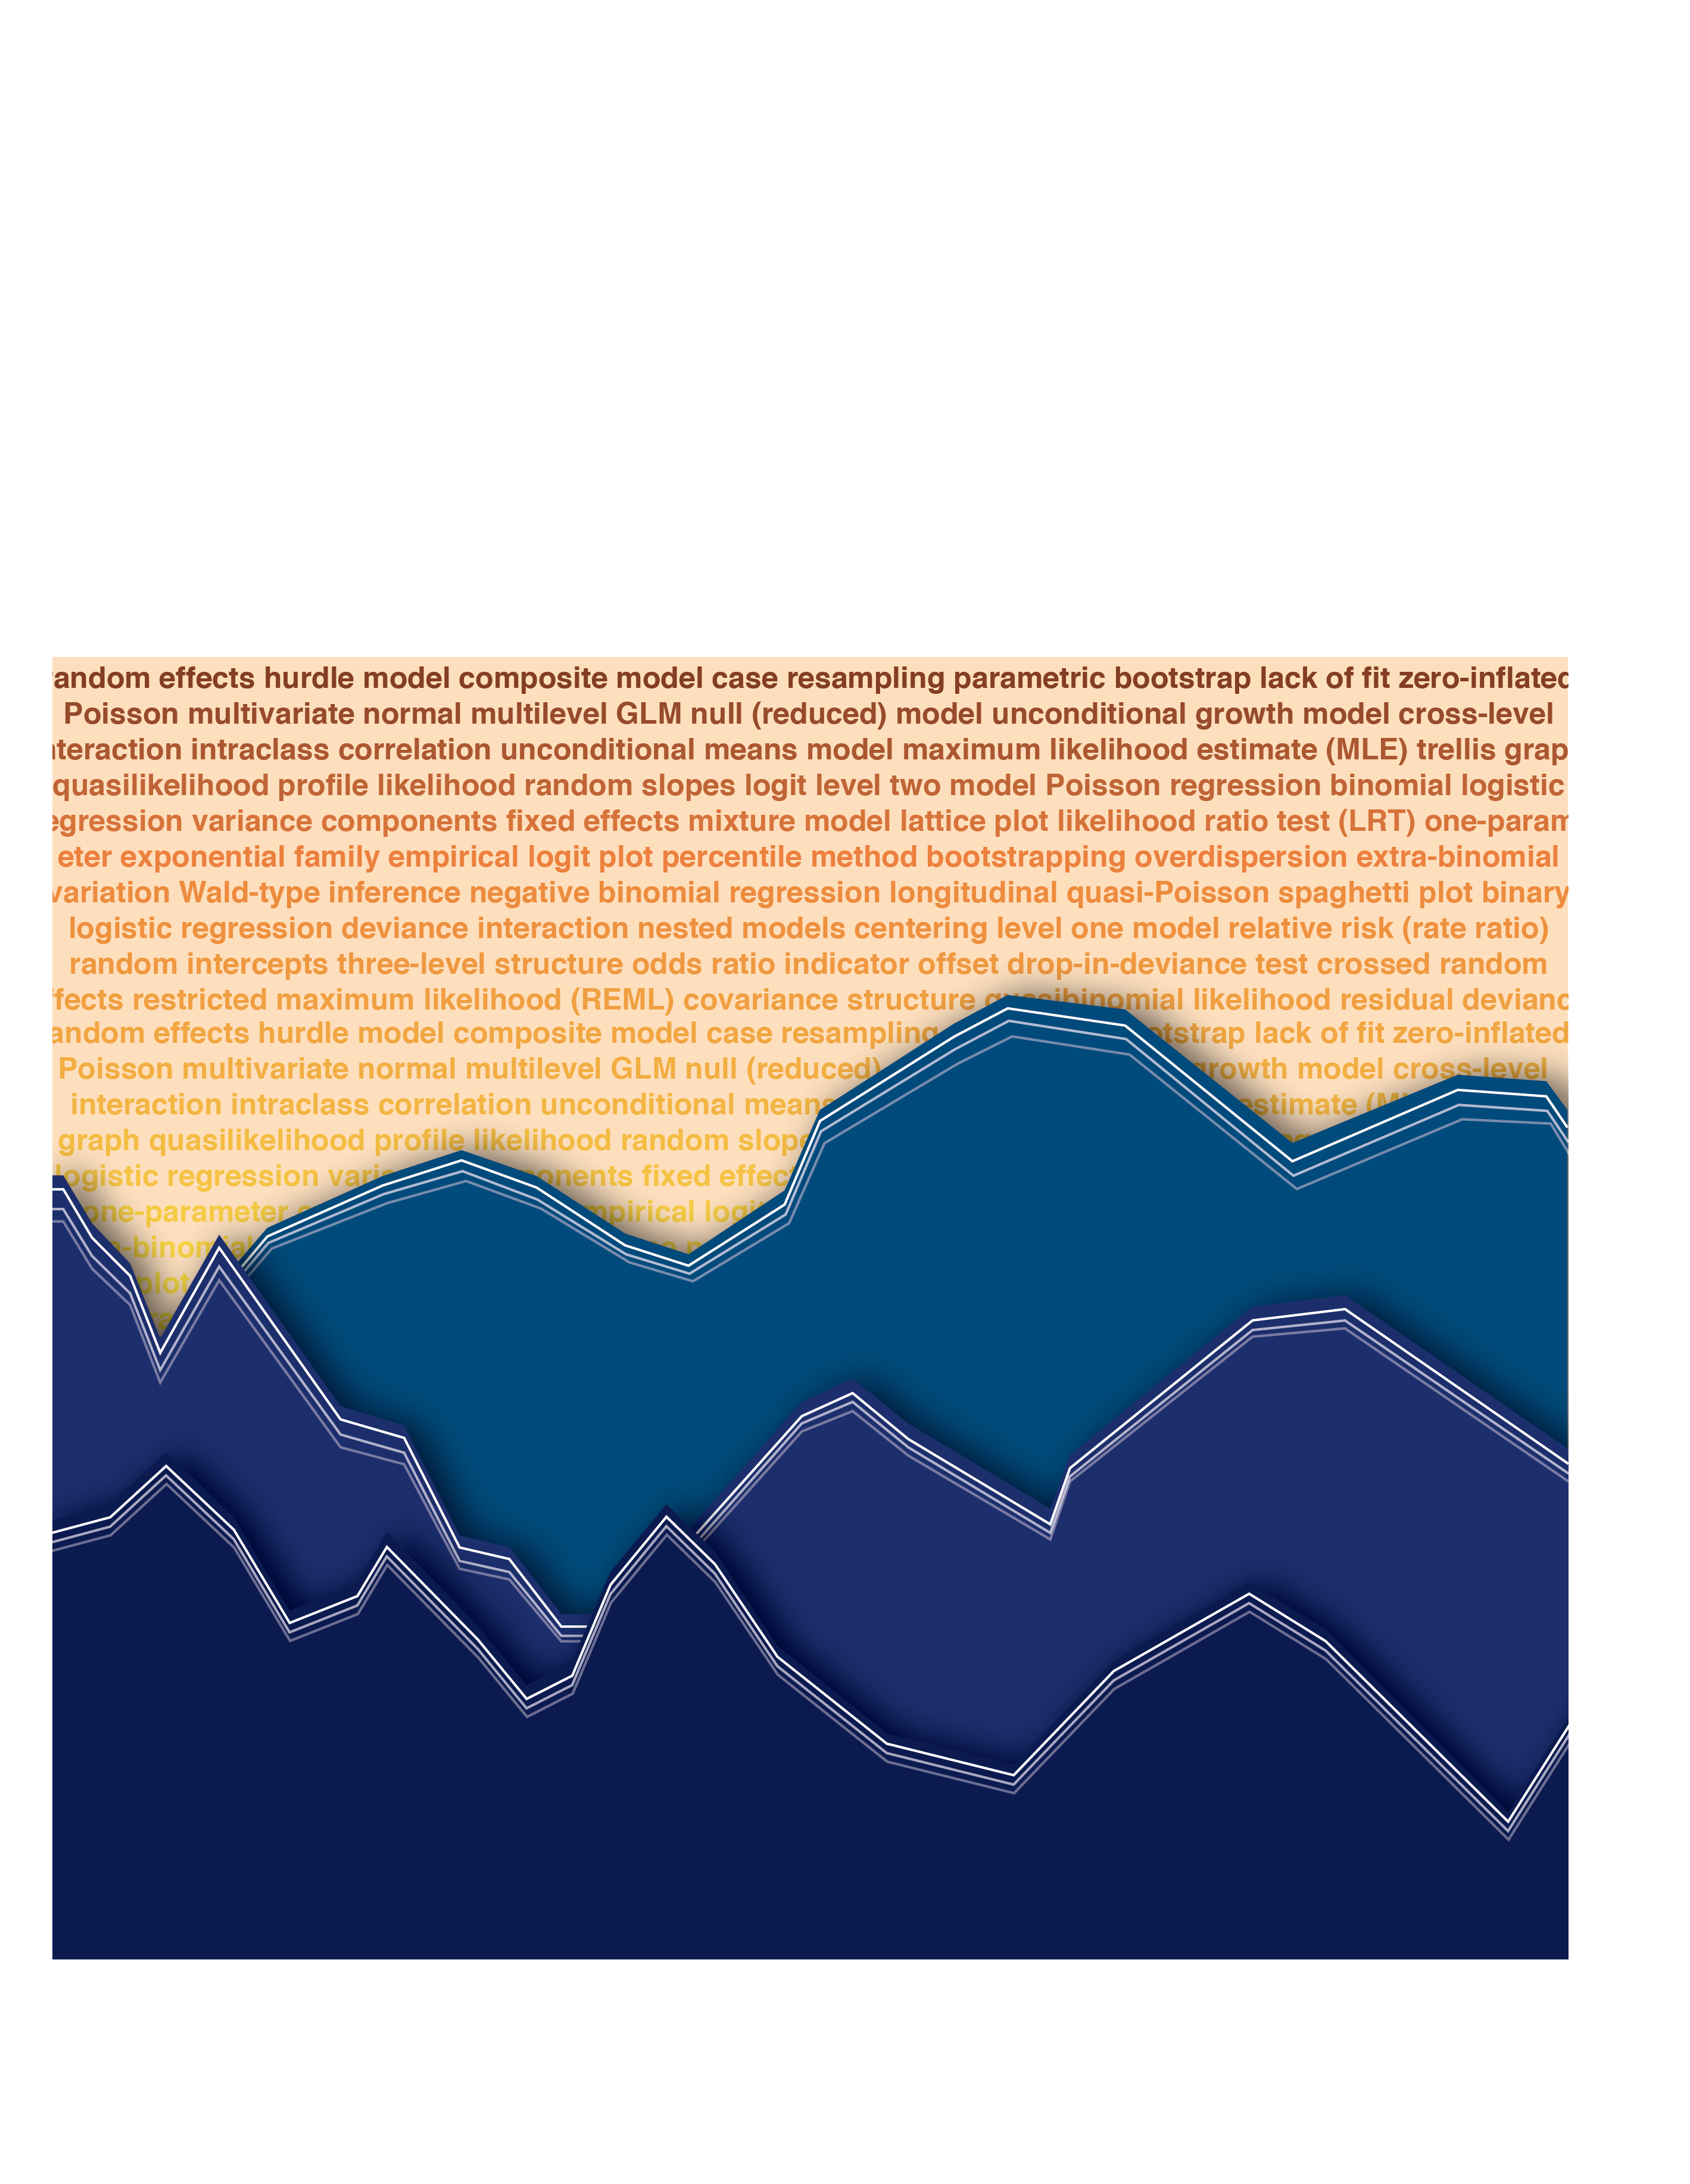
\includegraphics[width=0.75\linewidth]{data/cover}

\textbf{GLMs and Multilevel Models: Broadening Your Statistical Horizons (BYSH) with Applications using R} is intended to be accessible to undergraduate students who have successfully completed a regression course through, for example, a textbook like \emph{Stat2} \citep{Cannon2019}. We started teaching this course at St.~Olaf in 2003 so students would be able to deal with the non-normal, correlated world we live in. It has been offered at St.~Olaf every year since. Even though there is no mathematical prerequisite, we still introduce fairly sophisticated topics such as likelihood theory, zero-inflated Poisson, and parametric bootstrapping in an intuitive and applied manner. We believe strongly in case studies featuring real data and real research questions; thus, most of the data in the textbook and \href{https://github.com/proback/BYSH}{available at our GitHub repo} arises from collaborative research conducted by the authors and their students, or from student projects. Our goal is that, after working through this material, students will not necessarily be expert in these methods and associated theory, but that they will develop an expanded toolkit and a greater appreciation for the wider world of data and statistical modeling.

This work is licensed under a Creative Commons Attribution-NonCommercial-ShareAlike 4.0 International License.

\textbf{Acknowledgements.} We would like to thank students of Stat 316 at St.~Olaf College since 2010 for their patience as this book has taken shape with their feedback. We would especially like to thank these St.~Olaf students for their summer research efforts which significantly improved aspects of this book: Cecilia Noecker, Anna Johanson, Nicole Bettes, Kiegan Rice, Anna Wall, Jack Wolf, Josh Pelayo, Spencer Eanes, and Emily Patterson. Early editions of this book also benefitted greatly from feedback from instructors who used these materials in their classes, including Matt Beckman, Laura Boehm Vock, Beth Chance, Laura Chihara, Mine Dogucu, and Katie Ziegler-Graham. Finally, we have appreciated the support of two NSF grants (\#DMS-1045015 and \#DMS-0354308) and of our colleagues in Mathematics, Statistics, and Computer Science at St.~Olaf.

\hypertarget{ch-beyondmost}{%
\chapter{Beyond Least Squares: Using Likelihoods to Fit and Compare Models}\label{ch-beyondmost}}

\hypertarget{learning-objectives}{%
\section{Learning Objectives}\label{learning-objectives}}

After finishing this chapter, you should be able to:

\begin{itemize}
\tightlist
\item
  Describe the concept of a likelihood, in words.
\item
  Know and apply the Principle of Maximum Likelihood for a simple example.
\item
  Identify three ways in which you can obtain or approximate an MLE .
\item
  Use likelihoods to compare models.
\item
  Construct a likelihood for a simple model.
\end{itemize}

This text encourages you to broaden your statistical horizons by moving beyond independent, identically distributed, normal responses (iidN). This chapter on likelihood focuses on ways to fit models, determine estimates, and compare models for a wide range of types of responses, not just iidN data. In your earlier study of statistics, you fit simple linear models using ordinary least squares (OLS). Fitting those models assumes that the mean value of a response, Y, is linearly related to some variable, X. However, often responses are not normally distributed. For example, a study in education may involve scoring responses on a test as correct or incorrect. This binary response may be explained by the number of hours students spend studying. However we do not expect a variable which takes on only 0 or 1 to be a linear function of time spent studying (see Figure \ref{fig:logistic1}).

\begin{Shaded}
\begin{Highlighting}[]
\CommentTok{# Packages required for Chapter 2}
\KeywordTok{library}\NormalTok{(gridExtra)  }
\KeywordTok{library}\NormalTok{(knitr) }
\KeywordTok{library}\NormalTok{(mosaic)}
\KeywordTok{library}\NormalTok{(xtable)}
\KeywordTok{library}\NormalTok{(kableExtra)}
\KeywordTok{library}\NormalTok{(tidyverse) }
\end{Highlighting}
\end{Shaded}

\begin{figure}

{\centering 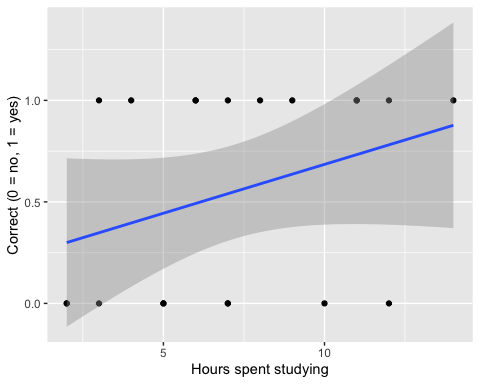
\includegraphics[width=0.9\linewidth]{bookdown-bysh_files/figure-latex/logistic1-1} 

}

\caption{An attempt to fit a linear regression model to a binary response variable.}\label{fig:logistic1}
\end{figure}

In this instance we'll use logistic regression instead of linear least squares regression. Fitting a logistic regression requires the use of likelihood methods. Another setting where likelihood methods come into play is when data is produced from a complex structure which may imply correlation among outcomes. For example, test scores for students who have been taught by the same teacher may be correlated. We'll see that likelihood methods are useful when modeling correlated data. Likelihood methods not only provide a great deal of flexibility in the types of models we can fit, but they also provide ways in which to compare models as well. You might find likelihood methods a bit more complicated, but conceptually the approach is straightforward. As you go through the material here, worry less about calculus and computational details and focus on the concepts. You will have software to help you with computation, but model specification and interpretation will be up to you.

\hypertarget{case-study-does-sex-run-in-families}{%
\section{Case Study: Does sex run in families?}\label{case-study-does-sex-run-in-families}}

Doesn't it seem that some families tend to have lots of boys while others have more than their share of girls? Is it really the case that each child human couples produce is equally likely to be a male or female? Or does sex run in families? It can be argued that these kinds of questions have implications for population demographics and sibling harmony. For example, a 2009 study at the University of Ulster found that growing up with sisters, as compared to brothers, can enhance the quality of life of an adult \citep{BBCNEWS1995}.

Sibling harmony aside, why do people care about gender imbalance? Comparisons of sex ratios between countries illustrate some compelling reasons. Some think that genetic or biological influences within families, such as ``sex running in families,'' can affect sex ratios. Mating behavior such as waiting until the family includes a boy or both sexes affects sex ratios. Some believe that sex ratios point to the practice of sex selection in a country accomplished through abortion or infanticide. Furthermore, there is speculation that an excess of men could lead to unrest among young males unable to find marriage partners or start families.

In 1930, statistician R.A. Fisher posited a 50:50 equilibrium theory regarding sex ratios in terms of parental expenditure. Most often, in practice, sex ratios differ from what Fisher predicted. From 1970 to 2002, the sex ratio at birth in the US among white non-Hispanics was 105 boys to 100 girls, but only 103 boys to 100 girls among African Americans and Native Americans \citep{Mathews2005}. A 1997 study in \emph{Nature} reports evidence which suggests that the human sex ratio may be currently shifting in the United States toward more female babies, closer to Fisher's prediction! \citep{Komdeur1997} Sex ratio comparisons between countries are also intriguing. For example, Switzerland has a sex ratio of 106 boys to 100 girls whereas there are 112 boys to every 100 girls in China acoording to The World Factbook \citep{CIA2013}. In the next section, we bring the notion of gender imbalance closer to home by focusing on families instead of countries or sub-populations.

To investigate this question and others, we look at the gender composition of 5,626 families collected by the National Longitudinal Survey of Youth \citep{NLSY1997}. We fit models to explore whether there is evidence sex runs in families, a model we refer to as a Sex Conditional Model. We also consider a separate but related question about whether couples are ``waiting for a boy.'' \citep{Rodgers2001}.

\hypertarget{research-questions}{%
\subsection{Research Questions}\label{research-questions}}

We specify several models related to gender balance in families. Our models liken having babies to flipping a coin (heads=boy, tails=girl), of course, recognizing that in truth there is a little more to having babies. The baseline model (Model 0) assumes that the probability of a boy is the same as a probability of a girl. The first model (Model 1) considers the situation that the coin is loaded and the probability of heads (a boy) is different than the probability of tails (a girl). Next, we consider a model (Model 2) that conditions on the previous number of boys or girls in a family to get at the question of whether sex runs in families. This data is also used for a different set of models that relate to couples' behavior. Specifically, we look to see if there is evidence that couples are waiting for a boy. searching for evidence of waiting for a girl, or waiting for both a boy and a girl, are left as exercises.

Models 0 and 1 assume that having children is like flipping a coin. The gender of each child is independent of the gender of other children and the probability of a boy is the same for each new child. Let \(p_B\) be the probability a child is a boy.

\begin{enumerate}
\def\labelenumi{\arabic{enumi}.}
\tightlist
\item
  \textbf{Model 0: Sex Unconditional Model (Equal probabilities)} Is a child just as likely to be a boy as it is to be a girl; is \(p_B\) = 0.5?
\item
  \textbf{Model 1: Sex Unconditional Model (Different probabilities)} Is the coin loaded; is \(p_B \neq 0.5\)?
\item
  \textbf{Model 2: Sex Conditional Model (Sex bias)}: Do boys or girls run in families? That is,
  is there a tendency for families with more boys than girls to be more likely to produce another boy? Is the case the same for girls?
\item
  \textbf{Model 3: Stopping Rule Model (Waiting for a boy)}
  Is there evidence that couples stop having children once a boy is born?
\end{enumerate}

Ultimately, our goal is to incorporate the family composition data represented as series of coin flips to find the ``best'' estimate for the probability of having a boy, \(p_B\), and evaluate the assumptions built into these models. We will be using likelihood-based methods, not ordinary least squares, to fit and compare these models.

While the NLSY data is of interest, we start with a smaller, hypothetical data set of 30 families with a total of 50 children in order to illustrate concepts related to likelihoods (Table \ref{tab:table1chp2}). The data are the frequencies of possible family gender compositions for one-, two-, and three-child families. The methods we develop on this small data set will then be applied to the one-, two- and three-family NLSY data. It is straightforward to include all of the family sizes up to the four-or five-child families in the NLSY data.

\begin{table}

\caption{\label{tab:table1chp2}The gender composition of 30 families in the hypothetical data set of n=50 children.}
\centering
\begin{tabular}[t]{lrr}
\toprule
Composition & Number of families & Number of children\\
\midrule
B & 6 & 6\\
G & 7 & 7\\
BB & 5 & 10\\
BG & 4 & 8\\
GB & 5 & 10\\
\addlinespace
GGB & 1 & 3\\
GBB & 2 & 6\\
Total & 30 & 50\\
\bottomrule
\end{tabular}
\end{table}

\hypertarget{model-0-sex-unconditional-model-equal-probabilities-independence}{%
\section{Model 0: Sex Unconditional Model (Equal probabilities, Independence)}\label{model-0-sex-unconditional-model-equal-probabilities-independence}}

For the Sex Unconditional models, having children is modeled using coin flips. With a coin flip model, the result of each flip is independent of results of other flips. With this version of the Sex Unconditional Model, the chance that a baby is a boy is specified to be \(p_B=0.5\). It makes no difference if the first and third children are boys, the probability that the second child is a boy is 0.5; that is, the results for each child are \textbf{independent} of the others. Under this model you expect to see equal numbers of boys and girls.

\hypertarget{sex_unconditional_model}{%
\section{Model 1: Sex Unconditional Model (Any Probability, Independence)}\label{sex_unconditional_model}}

You may want your model to allow for the probability of a boy, \(p_B\), to be something different than 0.5. With this version of the Sex Unconditional model, \(p_B>0.5\) or \(p_B<0.5\) or \(p_B=0.5\), in which case you expect to see more boys than girls or fewer boys than girls or equal numbers of boys and girls, respectively. We would retain the assumption of independence; that is, the probability of a boy, \(p_B\), is the same for each child. Seeing a boy for the first child will not lead you to change the probability that the second child is a boy; this would not imply that ``sex runs in families.''

\hypertarget{what-is-a-likelihood}{%
\subsection{What is a likelihood?}\label{what-is-a-likelihood}}

As is often the case in statistics, our objective is to find an estimate for a model parameter using our data; here, the parameter to estimate is the probability of a boy, \(p_B\), and the data is the gender composition for each family. One way in which to interpret probability is to imagine repeatedly producing children. The probability of a boy will be the overall proportion of boys as the number of children increases.
With likelihood methods, conceptually we consider different possible values for our parameter(s), \(p_B\), and determine how likely we would be to see our observed data in each case, \(\lik(p_B)\). We'll select as our estimate the value of \(p_B\) for which our data is most likely. A \textbf{likelihood} is a function that tells us how likely we are to observe our data for a given parameter value, \(p_B\). For a single family which has a girl followed by two boys, GBB, the likelihood function looks like:

\begin{equation}
 \lik (p_B) = P(G)P(B)P(B) = (1-p_B)p_B^2
 \label{eq:GBBlik}
\end{equation}

\begin{figure}

{\centering 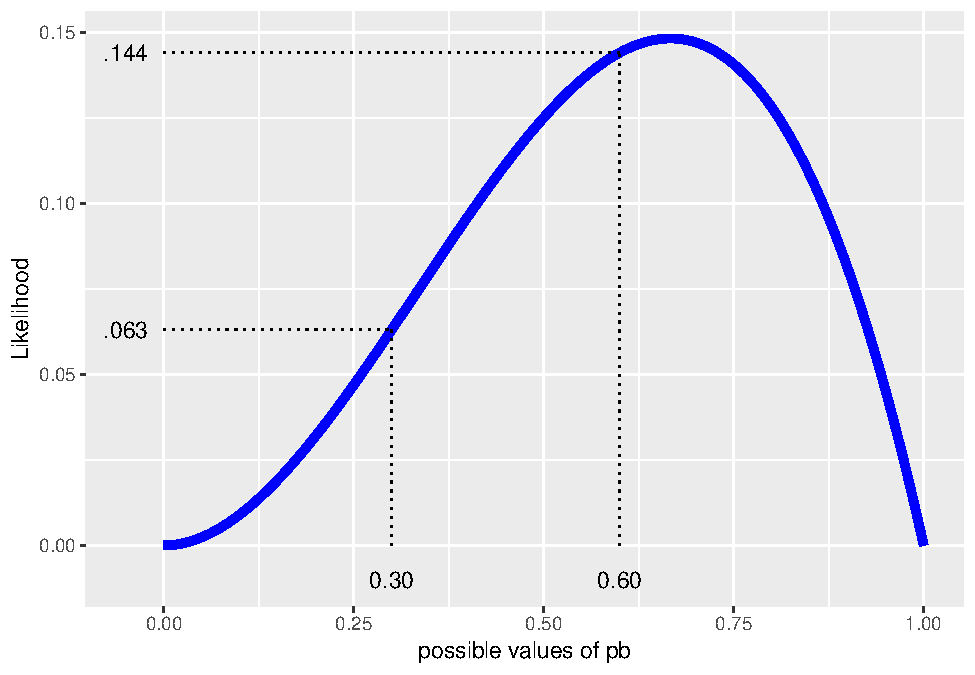
\includegraphics[width=0.9\linewidth]{bookdown-bysh_files/figure-latex/lik1-1} 

}

\caption{Likehood function for GBB.}\label{fig:lik1}
\end{figure}

From the likelihood in Figure \ref{fig:lik1}, when \(p_B\) = 0.3 we see a family of a girl followed by two boys 6.3\% (\(0.7\cdot0.3^2\)) of the time. However, it indicates that we are much more likely to see our data if \(p_B\) = 0.6 where the likelihood of GBB is \(0.4\cdot0.6^2\) or 14.4\%.

If the choice was between 0.3 and 0.6 for an estimate of \(p_B\), we'd choose 0.6. The ``best'' estimate of \(p_B\) would be the value where we are most likely to see our data from all possible values between 0 and 1, which we refer to as the \textbf{maximum likelihood estimate} or MLE. We can approximate an MLE using graphical or numerical approaches. Graphically, here it looks like the MLE is just above 0.6. In many, but not all, circumstances, we can obtain an MLE exactly using calculus. In this simple example, the MLE is 2/3. This is consistent with our intuition since 2 out of the 3 children are boys.

Suppose another family consisting of three girls is added to our data set. We've already seen that the Sex Unconditional Model multiplies probabilities to construct a likelihood because children are independent of one another. Extending this idea, families can be assumed to be independent of one another so that the likelihood for both families can be obtained by multiplication. With two families (GBB and GGG) our likelihood is now:

\begin{align*}
 \lik (p_B) &= P(GBB)P(GGG) \\
            &= [(1-p_B)p_B^2][(1-p_B)^3] \\
            &= (1-p_B)^4p_B^2
\end{align*}

A plot of this likelihood appears in Figure \ref{fig:lik2}. It is right skewed with an MLE at approximately 0.3. Using calculus, we can show that the MLE is precisely 1/3 which is consistent with intuition given the 2 boys and 4 girls in our data.

\begin{figure}

{\centering 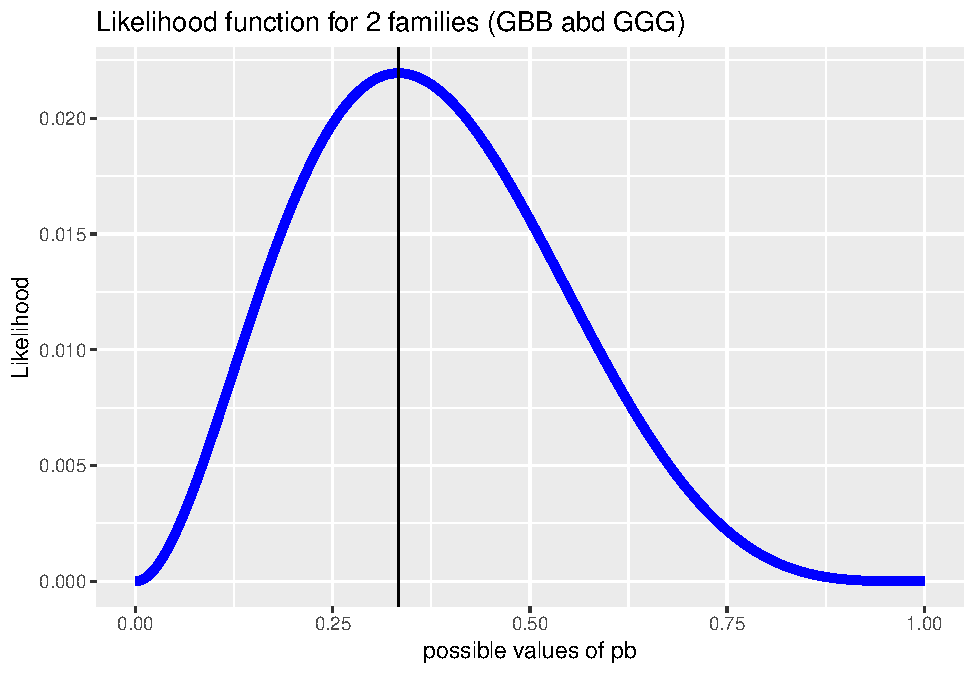
\includegraphics[width=0.9\linewidth]{bookdown-bysh_files/figure-latex/lik2-1} 

}

\caption{Likelihood function for the data of 2 families (GBB and GGG). The solid line is at the MLE,  ${p}_B=1/3$}\label{fig:lik2}
\end{figure}

Turning now to our hypothetical data with 30 families who have a total of 50 children, we can create the likelihood contribution for each of the family compositions.

\begin{table}

\caption{\label{tab:table2chp2}The likelihood factors for the hypothetical data set of n=50 children.}
\centering
\resizebox{\linewidth}{!}{
\begin{tabular}[t]{l>{\raggedright\arraybackslash}p{4cm}r>{\raggedright\arraybackslash}p{4cm}}
\toprule
Composition & Likelihood contribution for one family & Number of families & Likelihood contribution for multiple families\\
\midrule
B & $p_B$ & 6 & $p^6_B$\\
G & ($1-p_B$) & 7 & $(1-p_B)^7$\\
BB & $p^2_B$ & 5 & $p^{10}_B$\\
BG & $p_B(1-p_B)$ & 4 & $p^4_B(1-p_B)^4$\\
GB & $(1-p_B)p_B$ & 5 & $(1-p_B)^5 p^5_B$\\
\addlinespace
GGB & $(1-p_B)^2 p_B$ & 1 & $(1-p_B)^2 p_B$\\
GBB & $(1-p_B)p^2_B$ & 2 & $(1-p_B)^2 p^4_B$\\
Total &  & 30 & \\
\bottomrule
\end{tabular}}
\end{table}

The likelihood function for the hypothetical data set can be found by taking the product of the entries in the last column of Table \ref{tab:table2chp2} and simplifying.

\begin{equation}
\begin{split}
 \lik(p_B) &= p_B^{6}(1-p_B)^{7}p_B^{10} \cdots \\
 &= p_B^{30}(1-p_B)^{20}
\end{split}
 \label{eq:lik30}
\end{equation}

It should be obvious that the likelihood for this Sex Unconditional Model (the coin flipping model) has the simple form:

\begin{equation}
\lik(p_B) = p_B^{n_\textrm{Boys}}(1-p_B)^{n_\textrm{Girls}}
 \label{eq:lik30v2}
\end{equation}

and as we asserted above, the MLE will be the (number of boys)/(number of kids) or 30/50 here. Now, more formally, we demonstrate how we use the likelihood principle to approximate the MLE or determine it exactly.

\hypertarget{findMLE.sec}{%
\subsection{Finding MLEs}\label{findMLE.sec}}

\hypertarget{MLEgph.sec}{%
\subsubsection{Graphically approximating an MLE}\label{MLEgph.sec}}

\begin{figure}

{\centering 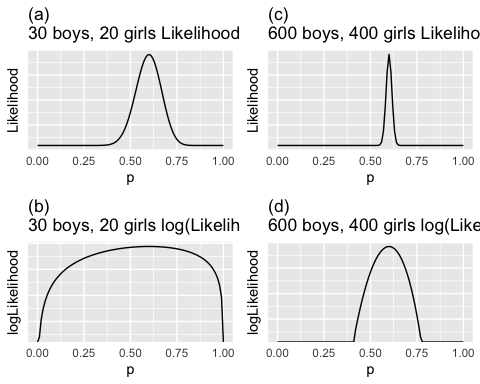
\includegraphics[width=0.9\linewidth]{bookdown-bysh_files/figure-latex/lik4-1} 

}

\caption{Likelihood and log-likelihood functions for 50 children (30 boys and 20 girls) and for 1000 children (600 boys and 400 girls).}\label{fig:lik4}
\end{figure}

Figure \ref{fig:lik4}(a) is the likelihood for the data set of 50 children. The height of each point is the likelihood and the possible values for \(p_B\) appear across the horizontal axis. It appears that our data is most likely when \(p_B = 0.6\) as we would expect. Note that the log of the likelihood function in Figure \ref{fig:lik4}(b) is maximized at the same spot: \(p_B = 0.6\); we will see advantages of using log likelihoods a bit later. Figures \ref{fig:lik4}(c) and (d) are also maximized at \(p_B = 0.6\), but they illustrate less variability and a sharper peak since there is more data (although the same proportions of boys and girls).

\hypertarget{numerically-approximating-an-mle}{%
\subsubsection{Numerically approximating an MLE}\label{numerically-approximating-an-mle}}

Here a grid search is used with the software package R to find maximum likelihood estimates, something that can be done with most software. A grid search specifies a set of finite possible values for \(p_B\) and then the likelihood, \(\Lik(p_B)\), is computed for each of the possible values. First, we define a relatively coarse grid by specifying 50 values for \(p_B\) and then computing how likely we would see our data for each of these possible values. The second example uses a finer grid, 1,000 values for \(p_B\), which allows us to determine a better (more precise) approximation of the MLE. In addition, most packages, like R, have an optimize function which can also be used to obtain MLEs. Both of these approaches are illustrated in the following code.

\begin{Shaded}
\begin{Highlighting}[]
\NormalTok{Lik.f <-}\StringTok{ }\ControlFlowTok{function}\NormalTok{(nBoys,nGirls,nGrid)\{}
    \CommentTok{# possible values for prob a boy is born}
\NormalTok{    pb <-}\StringTok{ }\KeywordTok{seq}\NormalTok{(}\DecValTok{0}\NormalTok{, }\DecValTok{1}\NormalTok{, }\DataTypeTok{length =}\NormalTok{ nGrid)   }
\NormalTok{    lik <-}\StringTok{ }\NormalTok{pb}\OperatorTok{^}\NormalTok{\{nBoys\} }\OperatorTok{*}\StringTok{ }\NormalTok{(}\DecValTok{1} \OperatorTok{-}\StringTok{ }\NormalTok{pb)}\OperatorTok{^}\NormalTok{\{nGirls\}}
    \CommentTok{# maximum likelihood over nGrid values of pb}
    \KeywordTok{max}\NormalTok{(lik)             }
    \CommentTok{# value of pb where likelihood maximized}
\NormalTok{    pb[lik}\OperatorTok{==}\KeywordTok{max}\NormalTok{(lik)]    }
\NormalTok{  \}}
\CommentTok{# estimated maximum likelihood estimator for p_B}
\KeywordTok{Lik.f}\NormalTok{(}\DataTypeTok{nBoys =} \DecValTok{30}\NormalTok{, }\DataTypeTok{nGirls =} \DecValTok{20}\NormalTok{, }\DataTypeTok{nGrid =} \DecValTok{50}\NormalTok{) }
\end{Highlighting}
\end{Shaded}

\begin{verbatim}
## [1] 0.5918
\end{verbatim}

\begin{Shaded}
\begin{Highlighting}[]
\CommentTok{# more precise MLE for p_B based on finer grid (more points)}
\KeywordTok{Lik.f}\NormalTok{(}\DataTypeTok{nBoys =} \DecValTok{30}\NormalTok{, }\DataTypeTok{nGirls =} \DecValTok{20}\NormalTok{, }\DataTypeTok{nGrid =} \DecValTok{1000}\NormalTok{)}
\end{Highlighting}
\end{Shaded}

\begin{verbatim}
## [1] 0.5996
\end{verbatim}

\begin{Shaded}
\begin{Highlighting}[]
\CommentTok{## Another approach: using R's optimize command}
\CommentTok{##   Note that the log-likelihood is optimized here}
\NormalTok{oLik.f <-}\StringTok{ }\ControlFlowTok{function}\NormalTok{(pb)\{}
    \KeywordTok{return}\NormalTok{(}\DecValTok{30}\OperatorTok{*}\KeywordTok{log}\NormalTok{(pb) }\OperatorTok{+}\StringTok{ }\DecValTok{20}\OperatorTok{*}\KeywordTok{log}\NormalTok{(}\DecValTok{1}\OperatorTok{-}\NormalTok{pb))}
\NormalTok{  \}}
\KeywordTok{optimize}\NormalTok{(oLik.f, }\DataTypeTok{interval=}\KeywordTok{c}\NormalTok{(}\DecValTok{0}\NormalTok{,}\DecValTok{1}\NormalTok{), }\DataTypeTok{maximum=}\OtherTok{TRUE}\NormalTok{)}
\end{Highlighting}
\end{Shaded}

\begin{verbatim}
## $maximum
## [1] 0.6
## 
## $objective
## [1] -33.65
\end{verbatim}

\hypertarget{calc-sec}{%
\subsubsection{MLEs using calculus (Optional)}\label{calc-sec}}

Calculus may provide another way to determine an MLE. Here, we can ascertain the value of \(p_B\) where the likelihood is a maximum by using the first derivative of the likelihood with respect to \(p_B\). We obtain the first derivative using the Product Rule, set it to 0, solve for \(p_B\), and verify that a maximum occurs there.

\begin{equation*}
\frac{d}{dp_B}p_B^{30}(1-p_B)^{20} = 30p_B^{29}(1-p_B)^{20}-p^{30}_B20(1-p_B)^{19} = 0
\end{equation*}

This approach would produce \(p_B = .60\) as we intuited earlier; however, we'll find that likelihoods can get a lot more complicated than this one and there is a simpler way to proceed. This simpler approach is based on the fact that the log of a likelihood is maximized at the same value of \(p_B\) as the likelihood. Likelihoods are typically products which require the application of the Product Rule when differentiating, whereas log-likelihoods are sums which are much easier to differentiate. In addition, likelihoods can become tiny with large data sets. So we can take the log of the likelihood, differentiate it, and find the value of \(p_B\) where the log-likelihood is a maximum and have the MLE for \(p_B\). We observed this visually in Figure \ref{fig:lik4}, where (a) and (b) are maximized at the same \(p_B\) (as are (c) and (d)). For the data set with 50 children:

\begin{align*}
 \lik(p_B)                      &= p_B^{30}(1-p_B)^{20} \\
 \log(\lik(p_B))                &= 30\log(p_B)+20\log(1-p_B) \\
 \frac{d}{dp_B} \log(\lik(p_B)) &= \frac{30}{p_B} - \frac{20}{1-p_B} = 0
 \label{eq:dlogLik50}
\end{align*}

It is now straightforward to determine that the log-likelihood is maximized when \(p_B = 3/5.\) We say that the MLE is \(\hat{p}_B = 0.6\). This is the exact estimate that was approximated above.

\hypertarget{how-does-sample-size-affect-the-likelihood}{%
\subsubsection{How does sample size affect the likelihood?}\label{how-does-sample-size-affect-the-likelihood}}

Consider two hypothetical cases under the Sex Unconditional Model:

\textbf{Hypothetical Case 1: n = 50 children with 30 boys and 20 girls} In previous sections, we found the MLE, \(\hat{p}_B=0.6.\)

\textbf{Hypothetical Case 2: n = 1000 children with 600 boys and 400 girls} Our earlier work suggests that the MLE here is also \(\hat{p}_B=0.6.\)

The graphs of the likelihoods and log-likelihoods for these two cases in Figure \ref{fig:lik4} give us an idea of how the increase in the sample size affects the precision of our estimates. The likelihoods and log-likelihoods for the two sample sizes have similar forms; however, the graphs with the larger sample size are much narrower, reflecting the greater precision we have with more data. With only 50 children there is a wide range of \(p_B\) values that lead to values of the log-likelihood near its maximum, so it's less clear what the optimal \(p_B\) is. As we have seen in statistics courses before, a larger sample size will result in less variation in our estimates, thereby affecting the power of hypothesis tests and the width of the confidence intervals.

\hypertarget{summary}{%
\subsection{Summary}\label{summary}}

Using likelihoods to find estimates of parameters is conceptually intuitive---select the estimate for your parameter where your data is most likely. Often MLEs make a lot of intuitive sense in the context of a problem as well; for example, here the MLE for the probability of a boy is the observed proportion of boys in the data. It may seem like a lot of work for such an obvious result, but MLEs have some nice, useful theoretical properties, and we'll see that many more complex models can be fit using the principle of maximum likelihood.

In summary, we constructed a likelihood that reflected features of our Sex Unconditional Model, then we approximated the parameter value for which our data is most likely using a graph or software, or we determined our optimal parameter value exactly using calculus. You may not be familiar with calculus, yet the concept is clear from the graphs: just find the value of \(p_B\) where the likelihood or log likelihood is a maximum. Our ``best'' estimate for \(p_B\), the MLE, is where our data is most likely to be observed.

Work to understand the \emph{idea} of a likelihood. Likelihoods are the foundation upon which estimates are obtained and models compared for most of this course. Do not be overly concerned with calculus and computation at this point.

\hypertarget{is-a-likelihood-a-probability-function-optional}{%
\subsection{Is a likelihood a probability function? (Optional)}\label{is-a-likelihood-a-probability-function-optional}}

No.~Even though we use probabilities to construct likelihoods, a likelihood is not a probability function. A probability function fixes parameter values and take as inputs possible outcomes, returning the probability of seeing different outcomes given the parameter value. For example, you flip a loaded coin which comes up heads 25\% of the time. After 5 flips, you observe the outcome of three heads and two tails. A \emph{probability function} provides the probability of observing (3H,2T) when \(p_H=0.25\). If you flip this same coin another 5 times and observe all tails (5T), the probability function provides the probability of (5T) when \(p_H=0.25\).

In contrast, a likelihood is constructed by fixing the data, say (3H,2T). It takes as input \emph{possible parameter values} and returns the probability of seeing the fixed data for each parameter value. For example, the likelihood will provide the chance of seeing the data (3H,2T) if \(p_H=0.6\), the chance of seeing the data (3H,2T) if \(p_H=0.3\), and so on. With the likelihood we can find the value of \(p_H\) where we are most likely to see our data.

\hypertarget{sex_conditional.sec}{%
\section{Model 2: Sex Conditional Model (Sex Bias)}\label{sex_conditional.sec}}

Our first research question involves determining whether sex runs in the family. Do families who already have boys tend to have more additional boys than expected by chance, and do families who already have girls tend to have more additional girls than expected by chance? What do you think? And how could we use a statistical model to investigate this phenomenon? There are a number of different ways to construct a model for this question. Here's one possibility.

\hypertarget{model-specification}{%
\subsection{Model Specification}\label{model-specification}}

Unlike the previous model, the \(p_B\) in a Sex Conditional Model \emph{depends} on existing family compositions. We introduce \textbf{conditional probabilities} and conditional notation to make the dependence explicit. One way to interpret the notation \(P(A|B)\) is the ``probability of A \emph{given} B has occurred.'' Another way to read this notation is the ``probability of A \emph{conditional} on B.'' Here, let \(\neutral\) represent the probability the next child is a boy given that there are equal numbers of boys and girls (sex-neutral) in the existing family. Let \(\bbias\) represent the probability the next child is a boy if the family is boy-biased; i.e., there are more boys than girls prior to this child. Similarly, let \(\gbias\) represent the probability the next child is a boy if the family is girl-biased; i.e., there are more girls than boys prior to this child.

Before we are mired in notation and calculus, let's think about how these conditional probabilities can be used to describe sex running in families. While we only had one parameter, \(p_B\), to estimate in the Sex Unconditional Model, here we have three parameters: \(\neutral\), \(\bbias\), and \(\gbias\). Clearly if all three of these probabilities are equal, the probability a child is a boy does not depend upon the existing gender composition of the family and there is no evidence of sex running in families. A conditional probability \(\bbias\) that is larger than \(\neutral\) suggests families with more boys are more likely to produce additional boys in contrast to families with equal boys and girls. This finding would support the theory of ``boys run in families.'' An analogous argument holds for girls. In addition, comparisons of \(\bbias\) and \(\gbias\) to the parameter estimate \(p_B\) from the Sex Unconditional Model may be interesting and can be performed using likelihoods.

While it may seem that including families with a single child (singletons) would not be helpful for assessing whether there is a preponderance of one sex or another in families, in fact singleton families would be helpful in estimating \(\neutral\) because singletons join ``neutral families.''

\begin{table}

\caption{\label{tab:table3chp2}Family contributions to the likelihood for a Sex Conditional Model using a hypothetical data set  of n=50 children from 30 families.}
\centering
\resizebox{\linewidth}{!}{
\begin{tabular}[t]{lllr}
\toprule
Composition & Likelihood contribution & Prior Status & Number of families\\
\midrule
B & $\neutral$ & neutral & 6\\
G & $(1-\neutral)$ & neutral & 7\\
BB & $(\neutral) (\bbias)$ & neutral, boy bias & 5\\
BG & $(\neutral) (1-\bbias)$ & neutral, boy bias & 4\\
GB & $(1-\neutral) (\gbias)$ & neutral, girl bias & 5\\
\addlinespace
GGB & $(1-\neutral) (1-\gbias) (\gbias)$ & neutral, girl bias, girl bias & 1\\
GBB & $(1-\neutral) (\gbias) (\neutral)$ & neutral, girl bias, neutral & 2\\
Total &  &  & 30\\
\bottomrule
\end{tabular}}
\end{table}

\hypertarget{application-to-hypothetical-data}{%
\subsection{Application to Hypothetical Data}\label{application-to-hypothetical-data}}

Using the family composition data for 50 children in the 30 families that appears in Table \ref{tab:table3chp2}, we construct a likelihood. The six singleton families with only one boy contribute \(\neutral^6\) to the likelihood and the seven families with only one girl contribute \(p_{G|N}^7\) or \((1-\neutral)^7\). {[}Why do we use \(1-\neutral\) instead of \(p_{G|N}\)?{]} There are five families with two boys each with probability \((\neutral)(\bbias)\) contributing:

\[
[(\neutral)(\bbias)]^{5}.
\]

We construct the likelihood using data from all 30 families assuming families are independent to get:

\begin{equation}
\begin{split}
 \lik(\neutral,\ \bbias,\ \gbias) &= 
 \big[(\neutral)^{17}
 (1-\neutral)^{15}
 (\bbias)^{5} \\
 &{}(1-\bbias)^{4}
 (\gbias)^{8}
 (1-\gbias) \big]
\end{split}
\label{eq:lik50}
\end{equation}

A couple of points are worth noting. First, there are 50 factors in the likelihood corresponding to the 50 children in these 30 families. Second, in the Sex Unconditional example we only had one parameter, \(p_{B}\); here we have three parameters. This likelihood does not simplify like the Sex Unconditional Model to one that is a product of only two powers: one of \(p_B\) and the other of \(1-p_B\). Yet, the basic idea we discussed regarding using a likelihood to find parameter estimates is the same. To obtain the MLEs, we need to find the combination of values for our three parameters where the data is most likely to be observed. Conceptually, we are trying different combinations of possible values for these three parameters, one after another, until we find \emph{the} combination where the likelihood is a maximum. It will not be as easy to graph this likelihood and we will need multivariable calculus to locate the optimal combination of parameter values where the likelihood is a maximum. In this text, we do not assume you know multivariable calculus, but we do want you to retain the concepts associated with maximum likelihood estimates. In practice, we use software to obtain MLEs.

With calculus, we can take partial derivatives of the likelihood with respect to each parameter assuming the other parameters are fixed. As we saw in Section \ref{calc-sec}, differentiating the log of the likelihood often makes things easier. This same approach is recommended here. Set each partial derivative to 0 and solve for all parameters simultaneously.

Knowing that it is easier to work with log-likelihoods, let's take the log of the likelihood we constructed in Equation \eqref{eq:lik50}.

\begin{multline*}
\log (\lik(\neutral,\ \bbias,\ \gbias)) = 
        17\log(\neutral)+15\log(1-\neutral) \\
        +5\log(\bbias)+4\log(1-\bbias) 
        +8\log(\gbias)+1\log(1-\gbias)
\end{multline*}

Taking a partial derivative with respect to \(\neutral\)

\begin{align*}
\frac{17}{\neutral}  - \frac{15}{1-\neutral}&=0 \\
\hat{p}_{B|N}&= \frac{17}{32} \\
&=0.53 \\
\end{align*}

This estimate follows naturally. First consider all of the children who enter into a family with an equal number of boys and girls. From Table \ref{tab:table3chp2}, we can see there are 32 such children (30 are first kids and 2 are third kids in families with 1 boy and 1 girl). Of those children, 17 are boys. So, given that a child joins a sex neutral family, the chance they are a boy is 17/32. Similar calculations for \(\bbias\) and \(\gbias\) yield:

\begin{align*}
 \hat{p}_{B|N} &= 17/32 = 0.53  \\  
 \hat{p}_{B|\textrm{B Bias}} &= 5/9 = 0.56  \\
 \hat{p}_{B|\textrm{G Bias}} &= 8/9 = 0.89  
\end{align*}

If we anticipate any ``sex running in families'' effect, we would expect \(p_{B|\textrm{B Bias}}\) to be larger than the the probability of a boy in the neutral setting, \(\neutral\). In our small hypothetical example, \(\hat{p}_{B|\textrm{B Bias}}\) is slightly greater than 0.53, providing light support for the ``sex runs in families'' theory when it comes to boys. What about girls? Do families with more girls than boys tend to have a greater probability of having a girl? We found that the MLE for the probability of a girl in a girl biased setting is 1-0.89=0.11. \footnote{Note: A nice property of MLEs is demonstrated here. We have the MLE for \(\gbias\), and we want the MLE of \(p_{G|\textrm{G Bias}}=1-\gbias\). We can get it by replacing \(\gbias\) with its MLE; i.e., \(\hat{p}_{G|\textrm{G Bias}}=1-\hat{p}_{B|\textrm{G Bias}}\). In mathematical terms, you can get the MLE of a function by applying the function to the original MLE.} This data does not provide evidence that girls run in families since \(\hat{p}_{G|G_{bias}} = 0.11 < \hat{p}_{G|N}=0.47\); there is a markedly lower probability of a girl if the family is already girl biased. This data is, however, hypothetical. Let's take a look at some real data and see what we find.

\hypertarget{case-study-analysis-of-the-nlsy-data}{%
\section{Case Study: Analysis of the NLSY data}\label{case-study-analysis-of-the-nlsy-data}}

\hypertarget{model-building-plan}{%
\subsection{Model Building Plan}\label{model-building-plan}}

You should now have a feel for using the Likelihood Principle to obtain estimates of parameters using family gender composition data. Next, these ideas will be applied to the NLSY data summarized in Table 2 of \citep{Rodgers2001}. In addition to considering the Sex Unconditional and Conditional Models, we investigate some models that incorporate choices couples may make about when to stop having more children.

\hypertarget{EDA.sec}{%
\subsection{Family Composition of Boys and Girls, NLSY: Exploratory Data Analysis}\label{EDA.sec}}

We begin by performing an exploratory data analysis aimed at shedding some light on our research questions. We are looking for clues as to which of our models is most plausible. The first statistic of interest is the proportion of boys in the sample. There are 5,416 boys out of the 10,672 children or a proportion of .507 boys. While this proportion is very close to .500, it is worth noting that a difference of .007 could be meaningful in population terms.

\begin{table}

\caption{\label{tab:table4chp2}Number of families and children in families with given composition in NLSY data. Sex ratio and proportion males are given by family size.}
\centering
\resizebox{\linewidth}{!}{
\begin{tabular}[t]{>{\raggedright\arraybackslash}p{3cm}>{\raggedleft\arraybackslash}p{3cm}>{\raggedleft\arraybackslash}p{3cm}>{\raggedright\arraybackslash}p{3cm}>{\raggedright\arraybackslash}p{3cm}}
\toprule
Family Composition & Number of families & Number of children & males : females & p\_B\\
\midrule
B & 930 & 930 & 97 boys to 100 girls & 0.494\\
G & 951 & 951 &  & \\
BB & 582 & 1164 & 104 boys to 100 girls & 0.511\\
BG & 666 & 1332 &  & \\
GB & 666 & 1332 &  & \\
\addlinespace
GG & 530 & 1060 &  & \\
BBB & 186 & 558 & 104 boys to 100 girls & 0.510\\
BBG & 177 & 531 &  & \\
BGG & 173 & 519 &  & \\
BGB & 148 & 444 &  & \\
\addlinespace
GBB & 151 & 453 &  & \\
GGB & 125 & 375 &  & \\
GBG & 182 & 546 &  & \\
GGG & 159 & 477 &  & \\
\bottomrule
\end{tabular}}
\end{table}

Table \ref{tab:table4chp2} displays family composition data for the 5,626 families with one, two, or three children in the NLSY data set. This dataset includes 10,672 children. Because our interest centers on the proportion of males, let's calculate sex ratios and proportions of males for each family size. For one-child families the male to female ratio is less than one (97 males:100 females) whereas both two- and three-child families have ratios of 104 boys to 100 girls, what we may expect in a population which favors males. While our research questions do not specifically call for these measures stratified by family size, it still provides us with an idea of gender imbalance in the data.

Table \ref{tab:table6chp2} provides insight into whether sex runs in families if the probability of a boy is 0.5. Simple probability suggests that the percentage of 2-child families with all the same sex would be 50\% (BB or GG vs.~BG or GB) but in our data we see only 45\%. For 3-child families, we have 8 possible orderings of boys and girls and so we would expect 2 out of the 8 orderings (25\%) to be of the same sex (BBB or GGG), but in fact 27\% have the same sex among the 3-children families. These results do not provide overwhelming evidence of sex running in families. There are some potentially complicating factors: the probability of a boy may not be 0.5 or couples may be waiting for a boy or a girl or both.

\begin{table}

\caption{\label{tab:table6chp2}Proportion of families in NLSY data with all the same sex by number of children in the family. Note that 1-child families are all homogeneous with respect to sex so we look at 2- and 3- child families.}
\centering
\resizebox{\linewidth}{!}{
\begin{tabular}[t]{lrrl}
\toprule
Number of children & Number of families & Number with all same sex & Percent with same sex\\
\midrule
Two Children & 2444 & 1112 & 45\%\\
Three Children & 1301 & 345 & 27\%\\
\bottomrule
\end{tabular}}
\end{table}

Table \ref{tab:table7chp2} contains the number of families by size and the percentage of those which are families with one boy who is last. Some of these families may have ``waited'' for a boy and then quit childbearing after a boy was born. We see the proportion of one child families with a boy is slightly less than the 50\% expected. We'd expect one out of four, or 25\%, of 2-child family configurations to have one boy last and there is 27\% in our dataset. Only 8.6\% of 3-child families have one boy last, but in theory we would expect one out of eight or 12.5\% of 3-child families to have one boy last. So if, in fact, the probability of a boy is 50\%, there does not appear to be evidence supporting the notion that families wait for a boy.

\begin{table}

\caption{\label{tab:table7chp2}Proportion of families in NLSY data with only one boy who is born last.}
\centering
\resizebox{\linewidth}{!}{
\begin{tabular}[t]{lrrl}
\toprule
Number of children & Number of families & Number with one boy last & Percent with boy last\\
\midrule
One Child & 1881 & 930 & 49.4\%\\
Two Children & 2444 & 666 & 27.2\%\\
Three Children & 1301 & 125 & 8.6\%\\
\bottomrule
\end{tabular}}
\end{table}

There are many other ways to formulate and explore the idea that sex runs in families or that couples wait for a boy (or a girl). See \citet{Rodgers2001} for other examples.

\hypertarget{likelihood-for-the-sex-unconditional-model-the-nlsy-data}{%
\subsection{Likelihood for the Sex Unconditional Model: the NLSY data}\label{likelihood-for-the-sex-unconditional-model-the-nlsy-data}}

We construct a likelihood for the Sex Unconditional Model for the one-, two- and three-child families from the NLSY. See Table \ref{tab:table4chp2} for the frequencies of each gender composition.

Families with different compositions will contribute different factors to the likelihood. For example, Table \ref{tab:sexuncondmodel} shows a sample of contributions for a few family compositions, where coefficients come from Table \ref{tab:table4chp2}.

\begin{table}

\caption{\label{tab:sexuncondmodel}Contributions to the likelihood function for a sample of family compositions from the NLSY data}
\centering
\resizebox{\linewidth}{!}{
\begin{tabular}[t]{>{\raggedright\arraybackslash}p{5cm}>{\raggedright\arraybackslash}p{5cm}}
\toprule
Family composition & Likelihood contribution\\
\midrule
G & $(1-p_B)^{951}$\\
GB & $(1-p_B)^{666}p_B^{666}$\\
BGB & $p_B^{2*148}(1-p_B)^{148}$\\
\bottomrule
\end{tabular}}
\end{table}

Now we create the entire likelihood for our data under the Sex Unconditional Model.

\begin{align*}
 \Lik(p_B) &= p_B^{930}p_G^{951}p_{BB}^{582} \cdots p_{BBG}^{177} \cdots p_{GGG}^{159} \\
 &= p_B^{930+2*582+666+666+\cdots+182}(1-p_B)^{951+666+666+2*530+\cdots+3*159} \\
 &=  p_B^{5416}(1-p_B)^{5256} \\
 \label{eq:likSexUn}
\end{align*}

This very simple likelihood implies that each child contributes a factor of the form \(p_B\) or \(1-p_B\). Given that there are 10,672 children, what would be your best guess of the estimated probability of a boy for this model? We can determine the MLE for \(p_B\) using our previous work.

\begin{align}
 \hat{p_B} &= \frac{nBoys}{nBoys + nGirls} \\
 & =  \frac{5416}{5416+5256} \\
 &= 0.507
 \label{eq:MLESexUn}
\end{align}

\hypertarget{sex_cond_lik.sec}{%
\subsection{Likelihood for the Sex Conditional Model}\label{sex_cond_lik.sec}}

The contribution to a Sex Conditional Model likelihood for the same family compositions we considered in the previous section appear here.

\begin{quote}
G \((1-\neutral)^{951}\)\\
GB \((1-\neutral)^{666}\gbias^{666}\)\\
BGB \(\neutral^{2*148}(1-\bbias)^{148}\)
\end{quote}

The products of the last three columns of Table \ref{tab:table8chp2} provide the likelihood contributions for the Sex Conditional Model for all of the one-, two- and three-child NLSY families. We write the likelihood as a function of the three parameters \(\neutral, \bbias\), and \(\gbias\).

\begin{table}

\caption{\label{tab:table8chp2}Likelihood contributions for families in Sex Unconditional and Sex Conditional Models.}
\centering
\resizebox{\linewidth}{!}{
\begin{tabular}[t]{llllll}
\toprule
\multicolumn{1}{c}{ } & \multicolumn{1}{c}{ } & \multicolumn{1}{c}{ } & \multicolumn{3}{c}{Sex Conditional Model} \\
\cmidrule(l{3pt}r{3pt}){4-6}
Family composition & Number of families & Sex Unconditional & Child1 & Child 2 & Child 3\\
\midrule
B & 930 & $p_B$ & $\neutral$ &  & \\
G & 951 & $(1-p_B)$ & $1-\neutral$ &  & \\
BB & 582 & $p_B^2$ & $\neutral$ & $\bbias$ & \\
BG & 666 & $p_B (1-p_B)$ & $\neutral$ & $1-\bbias$ & \\
GB & 666 & $(1-p_B)p_B$ & $1-\neutral$ & $\gbias$ & \\
\addlinespace
GG & 530 & $(1-p_B)^2$ & $1-\neutral$ & $1-\gbias$ & \\
BBB & 186 & $p_B^3$ & $\neutral$ & $\bbias$ & $\bbias$\\
BBG & 177 & $p_B^2 (1-p_B)$ & $\neutral$ & $\bbias$ & $1-\bbias$\\
BGG & 173 & $p_B (1-p_B)^2$ & $\neutral$ & $1-\bbias$ & $1-\neutral$\\
BGB & 148 & $p_B^2 (1-p_B)$ & $\neutral$ & $1-\bbias$ & $\neutral$\\
\addlinespace
GBB & 151 & $p_B^2 (1-p_B)$ & $1-\neutral$ & $\gbias$ & $\neutral$\\
GGB & 125 & $p_B (1-p_B)^2$ & $1-\neutral$ & $1-\gbias$ & $\gbias$\\
GBG & 182 & $p_B(1-p_B)^2$ & $1-\neutral$ & $\gbias$ & $1-\neutral$\\
GGG & 159 & $(1-p_B)^3$ & $1-\neutral$ & $1-\gbias$ & $1-\gbias$\\
log-likelihood &  & -7396.067 &  & -7374.238 & \\
\addlinespace
AIC &  & 14794.13 &  & 14751.48 & \\
BIC &  & 14810.68 &  & 14749.18 & \\
\bottomrule
\end{tabular}}
\end{table}

\begin{align}
 \Lik(\neutral,  \bbias, \gbias)& = \big[ \neutral^{930}(1-\neutral)^{951} ( \neutral\bbias)^{582}\\
& \cdots  ((1-\neutral)(1-\gbias)(1-\gbias))^{159} \big]\\ 
&= \big[\neutral^{3161}(1-\neutral)^{3119}\bbias^{1131} \\
&    (1-\bbias)^{1164}\gbias^{1124}(1-\gbias)^{973} \big]\\
\label{eq:likall}
\end{align}

\begin{align}
\log(\Lik(\neutral,  \bbias, \gbias)) &= 3161\log(\neutral)+3119\log(1-\neutral)\\ 
 & {}+1131\log(\bbias)+1164\log(1-\bbias)\\   
 & {}+1124\log(\gbias)+ 973\log(1-\gbias)\\
\label{eq:log-likall} 
\end{align}

To use calculus to estimate the probability of a boy entering a neutral family (a family with equal boys and girls), \(\neutral\), we begin with the logarithm of the likelihood in equation \eqref{eq:log-likall}. Differentiating the log-likelihood with respect to \(\neutral\) holding all other parameters constant yields an intuitive estimate.

\begin{align*}
 \hat{p}_{B|N}&=\frac{3161}{3161+3119} \\
 &=0.5033
\end{align*}

There are 6,280 times when a child is joining a neutral family and of those times 3,161 are boys. Thus the MLE of the probability of a boy joining a family where the number of boys and girls are equal (including when there are no children) is 0.5033.

Similarly, MLEs for \(\bbias\) and \(\gbias\) can be obtained:
\begin{align*}
 \hat{p}_{B|\textrm{B Bias}}&= \frac{1131}{1131+1164}\\
 & =  0.4928 \\
 &  \\
 \hat{p}_{B|\textrm{G Bias}}&=\frac{1124}{1124+973}\\
&= 0.5360
\end{align*}

Are these results consistent with the notion that boys or girls run in families? We consider the Sex Conditional Model because we hypothesized there would be a higher probability of boys among children born into families with a boy bias. However, we found that if there is a boy bias the probability of a subsequent boy was estimated to be actually less, 0.493. Similarly, girls join families with more girls than boys approximately 46.4\% of the time so that there is little support for the idea that either ``girls or boys run in families.''

Even though initial estimates don't support the idea, let's formally take a look as to whether prior gender composition affects the probability of a boy. To do so, we'll see if the Sex Conditional Model is statistically significantly better than the Sex Unconditional Model.

\hypertarget{sec-lrtest}{%
\subsection{Comparing the Sex Unconditional to the Sex Conditional Model}\label{sec-lrtest}}

\hypertarget{nested-models}{%
\subsubsection{Nested Models}\label{nested-models}}

Likelihoods are not only useful for fitting models, but they are also useful when comparing models. If the parameters for a reduced model are a subset of parameters for a larger model, we say the models are \textbf{nested} and the difference between their likelihoods can be incorporated into a statistical test to help judge the benefit of including additional parameters. Another way in which to think of nesting is to consider whether parameters in the larger model can be equated to obtain the simpler model or whether some parameters in the larger model can be set to constants. Since \(\bbias, \neutral\) and \(\gbias\) in the Sex Conditional Model can be set to \(p_B\) to obtain the Sex Unconditional Model, we can say the models are nested.

If the parameters are not nested, comparing models with the likelihood can still be useful but will take a different form. We'll see that the Akaike Information Criterion (AIC) and Bayesian Information Criterion (BIC) are functions of the log-likelihood that can be used to compare models even when the models are not nested. Either way we see that this notion of likelihood is pretty useful.

\textbf{Hypotheses}

\(H_0: \neutral=\bbias=\gbias=p_B\) (Sex Unconditional Model)
The probability of a boy does not depend on the prior family composition.

\(H_A:\) At least one parameter from \(\neutral, \bbias,\gbias\) differs from the others. (Sex Conditional Model)
The probability of a boy does depend on the prior family composition.

We start with the idea of comparing the likelihoods or, equivalently, the log-likelihoods of each model at their maxima. To do so, we use the log-likelihoods to determine the MLEs, and then replace the parameters in the log-likelihood with their MLEs, thereby finding the maximum value for the log-likelihood of each model. Here we will refer to the first model, the Sex Unconditional Model, as the \textbf{reduced model} noting that it has only a single parameter, \(p_B\). The more complex model, the Sex Conditional Model, has three parameters and is referred to here as the \textbf{larger model}. We'll use the MLEs derived earlier. (Equations \eqref{eq:MLESexUn} and \eqref{eq:likall}).

The maximum of the log-likelihood for the reduced model can be found by replacing \(p_{B}\) in the log-likelihood with the MLE of \(p_{B}\), 0.5075.

\begin{align*}
\log(\Lik(0.5075))& = 5416\log(.5075) + 5256\log(1-.5075)\\
&= -7396.067\\
\end{align*}

The maximum of the log-likelihood for the larger model can be found by replacing \(\neutral, \bbias, \gbias\) in the log-likelihood with 0.5033, 0.4928, and 0.5360, respectively.

\begin{align*}
 \log(\Lik(0.5033, 0.4928, 0.5360)) &=  3161\log(.5033)+3119\log(1-.5033)\\
 & {}+ 1131\log(.4928)+1164\log(1-.4928)\\
 & {}+ 1124\log(.5360)+973\log(1-.5360)\\
 &= -7391.448
\end{align*}

Take a look at the log-likelihoods---the maximum log-likelihood for the larger model is indeed larger (less negative). The maximum log-likelihood for the larger model is guaranteed to be at least as large as the maximum log-likelihood for the reduced model, so we'll be interested in whether this observed difference in maximum log-likelihoods, -7391.448 -(-7396.067) = 4.619, is significant.

A result from statistical theory states that, when the reduced model is the true model, twice the difference of the maximum log-likelihoods follows a \(\chi^2\) distribution with the degrees of freedom equal to the difference in the number of parameters between the two models. A difference of the maximum log-likelihoods can also be looked at as the log of the ratio of the likelihoods and for that reason the test is referred to as the \textbf{Likelihood Ratio Test (LRT)}.

Our test statistic is

\begin{align}    
 \textrm{LRT} &= 2[\max(\log(\Lik(\textrm{larger model}))) - \max(\log(\Lik(\textrm{reduced model})))] \\
     &= 2\log\left(\frac{\max(\Lik(\textrm{larger  model}))}{\max(\Lik(\textrm{reduced model}))} \right)
\end{align}

Intuitively, when the likelihood for the larger model is much greater than it is for the reduced model, we have evidence that the larger model is more closely aligned with the observed data. This isn't really a fair comparison on the face of it. We need to account for the fact that more parameters were estimated and used for the larger model. That is accomplished by taking into account the degrees of freedom for the \(\chi^2\) distribution. The expected value of the \(\chi^2\) distribution is its degrees of freedom. Thus when the difference in the number of parameters is large, the test statistic will need to be much larger to convince us that it is not simply chance variation with two identical models. Here, under the reduced model we'd expect our test statistic to be 2, when in fact it is over 9. The evidence favors our larger model. More precisely, the test statistic is \(2(-7391.448+7396.073) = 9.238,\; (p=.0099)\).

We have convincing evidence that the Sex Conditional Model provides a significant improvement over the Sex Unconditional Model. However, keep in mind that our point estimates for a probability of a boy were not what we had expected for ``sex runs in families.'' It may be that this discrepancy stems from behavioral aspects of family formation. The next section on stopping rules explores how types of couples' decisions may affect the relative proportions of family compositions in the data.

\emph{Note: }You may notice that the LRT is similar in spirit to the extra-sum-of-squares F-test used in linear regression. Recall that the extra-sum-of-squares F-test involves comparing two nested models. When the smaller model is true, the F-ratio follows an F-distribution which on average is 1.0. A large, unusual F-ratio provides evidence that the larger model provides a significant improvement.

\emph{Also note: } It might have been more logical to start by using Likelihood Ratio Test to determine whether the probability of having a boy differs significantly from 0.5. We leave this as an exercise.

\hypertarget{model-3-stopping-rule-model-waiting-for-a-boy}{%
\section{Model 3: Stopping Rule Model (Waiting for a boy)}\label{model-3-stopping-rule-model-waiting-for-a-boy}}

\citet{Rodgers2001} offer one reason to explain the contradictory results: waiting for a male child. It has been noted by demographers that some parents are only interested in producing a male heir so that the appearance of a boy leads more often to the family ending childbearing. Stopping models investigate questions like: Are couples more likely to stop childbearing once they have a boy? Or are some parents waiting for a girl? Others might wish to have at least one boy and girl. The exploratory data analysis results in Table \ref{tab:table7chp2} provide some insight but cannot definitively settle the question about couples' stopping once they have a boy.

For stopping models, two probabilities are recorded for each child: the probability of the sex and the conditional probability of stopping after that child. As we have done in previous models, let \(p_B\) = probability the child is a boy. When conditioning, every possible condition must have a probability associated with it. Here the stopping conditions for Model 3 are: stop on first boy \((S|B1)\) or stopping on a child who is not the first boy \((S|N)\).

\textbf{Additional Parameters for the First Boy Stopping Model}

\begin{quote}
\(\bstop =\) probability of stopping after the first boy
\end{quote}

\begin{quote}
\(1 - \bstop=\) probability of not stopping after the first boy
\end{quote}

\begin{quote}
\(\nstop=\) probability of stopping after a child who is not the first boy
\end{quote}

\begin{quote}
\(1 - \nstop=\) probability of not stopping after a child who is not the first boy
\end{quote}

Our interest centers on whether the probability of stopping after the first boy, \(\bstop\) is greater than stopping when it is not a first boy, \(\nstop\).

\begin{table}

\caption{\label{tab:table9chp2}Likelihood contributions for families in Model 3: Waiting for a boy.}
\centering
\resizebox{\linewidth}{!}{
\begin{tabular}[t]{lrll}
\toprule
Family Composition & Number of families &   Likelihood & Contribution\\
\midrule
B & 930 & $p_B$ & $\bstop$\\
G & 951 & $(1-p_B)$ & $\nstop$\\
BB & 582 & $p_B^2$ & $(1-\bstop) \nstop$\\
BG & 666 & $p_B (1-p_B)$ & $(1-\bstop) \nstop$\\
GB & 666 & $(1-p_B)p_B$ & $(1-\nstop) \bstop$\\
\addlinespace
GG & 530 & $(1-p_B)^2$ & $(1-\nstop)\nstop$\\
BBB & 186 & $p_B^3$ & $(1-\bstop) (1-\nstop)\nstop$\\
BBG & 177 & $p_B^2 (1-p_B)$ & $(1-\bstop) (1-\nstop)\nstop$\\
BGG & 173 & $p_B (1-p_B)^2$ & $(1-\bstop) (1-\nstop)\nstop$\\
BGB & 148 & $p_B^2 (1-p_B)$ & $(1-\bstop) (1-\nstop)\nstop$\\
\addlinespace
GBB & 151 & $p_B^2 (1-p_B)$ & $(1-\nstop) (1-\bstop)\nstop$\\
GGB & 125 & $p_B (1-p_B)^2$ & $(1-\nstop)^2 \bstop$\\
GBG & 182 & $p_B(1-p_B)^2$ & $(1-\nstop) (1-\bstop)\nstop$\\
GGG & 159 & $(1-p_B)^3$ & $(1-\nstop)^2 \nstop$\\
\bottomrule
\end{tabular}}
\end{table}

\begin{table}

\caption{\label{tab:table10chp2}Patterns related to stopping decisions.}
\centering
\begin{tabular}[t]{lllll}
\toprule
Child is... & total children & prop of all children & n.stops (n.families) & prop stopped after these children\\
\midrule
a boy who is the only boy in the family up to that point & 3,986 & 37.4\% & 1,721 & 43.2\%\\
not an only boy in the family up to that point & 6,686 & 62.2\% & 3,905 & 58.4\%\\
a girl who is the only girl in the family up to that point & 3,928 & 36.8\% & 1,794 & 45.7\%\\
not an only girl in the family up to that point & 3,832 & 63.2\% & 3,832 & 56.8\%\\
 & 10,672 &  & 5,626 & \\
\bottomrule
\end{tabular}
\end{table}

Using calculus, the MLEs are derived to be \(\hat{p}_B = 0.507\), \(\hat{p}_{S|B1} = 0.432\), and \(\hat{p}_{S|N} = 0.584\). These are consistent with intuition. The estimated proportion of boys for this model is the same as the estimate for the Sex Unconditional Model (Model 1). The estimates of the stopping parameters are consistent with the fact that of the 3,986 first boys, parents stop 43.2\% of the time and of the 6,686 children who are not first boys childbearing stopped 58.4\% of the time. See Table \ref{tab:table10chp2}

These results do, in fact, suggest that the probability a couple stops childbearing on the first boy is different than the probability of stopping at a child who is not the first boy, but the direction of the difference does not imply that couples ``wait for a boy,'' rather it appears that they are less likely to stop childbearing after the first boy in comparison to children who are not the first born male.

Similarly, for girls, the MLEs are \(\hat{p}_{S|G1}\) = 0.457 and \(\hat{p}_{S|N}\) = 0.568. Once again, the estimates do not provide evidence of waiting for a girl.

\hypertarget{non-nested-models}{%
\subsection{Non-nested Models}\label{non-nested-models}}

How does the waiting for a boy model compare to the waiting for a girl model? Thus far we've seen how nested models can be compared. But these two models are not nested. Two measures referred to as information criteria, AIC and BIC, are useful when comparing non-nested models. Each measure can be calculated for a model using a function of the model's maximum log-likelihood. You can find the log-likelihood in the output from most modeling software packages.

\begin{itemize}
\tightlist
\item
  \(\textrm{AIC} = -2 (\textrm{maximum log-likelihood }) + 2p\), where \(p\) represents the number of parameters in the fitted model. AIC stands for Akaike Information Criterion. Because smaller AICs imply better models, we can think of the second term as a penalty for model complexity---the more variables we use the larger the AIC.
\item
  \(\textrm{BIC} = -2 (\textrm{maximum log-likelihood }) + p\log(n)\), where \(p\) is the number of parameters and \(n\) is the number of observations. BIC stands for Bayesian Information Criterion, also known as Schwarz's Bayesian criterion (SBC). Here we see that the penalty for the BIC differs from the AIC, where the log of the number of observations heavily penalizes models built with large datasets.
\end{itemize}

So which explanation of the data seems more plausible---waiting for a boy or waiting for a girl? These models are not nested (i.e., one is not a simplified version of the other), so it is not correct to perform a Likelihood Ratio Test, but we can legitimately compare these models using information criteria.

\begin{table}

\caption{\label{tab:tab1chp2}Measures of model performance: Waiting for a Boy vs. Waiting for a Girl Model.}
\centering
\begin{tabular}[t]{lrr}
\toprule
  & Waiting for a boy & Waiting for a girl\\
\midrule
max log-likelihood & -14661 & -14716\\
AIC & 29324 & 29433\\
BIC & 29332 & 29441\\
\bottomrule
\end{tabular}
\end{table}

Smaller AIC and BIC are preferred, so here the Waiting for a Boy Model is judged superior to the Waiting for a Girl Model suggesting that couples waiting for a boy is a better explanation of the data than waiting for a girl. However, for either boys and girls, couples do not stop more frequently after the first occurrence.

Other stopping rule models are possible. Another model could be that couples wait to stop until they have both a boy and a girl. We leave the consideration of this balance-preference model as an exercise.

\hypertarget{summary-of-model-building}{%
\section{Summary of Model Building}\label{summary-of-model-building}}

Using a Likelihood Ratio Test, we found statistical evidence that the Sex Conditional Model (Sex Bias) is preferred to the Sex Unconditional Models. However, the parameter estimates were not what we expected if we believe that sex runs in families. Quite to the contrary, the results suggested that if there were more of one sex in a family, the next child is likely to be of the other sex. The results may support the idea that gender composition tends to ``even out'' over time.

Using AICs and BICs to compare the non-nested models of waiting for a boy or waiting for a girl, we found that the model specifying stopping for a first boy was superior to the model for stopping for the first girl. Again, neither model suggested that couples were \emph{more} likely to stop after the first male or female, rather it appeared just the opposite---couples were \emph{less} likely to be stopping after the first boy or first girl.

These results may need to be considered conditional on the size of a family. In which case, a look at the exploratory data analysis results may be informative. The reported percentages in Table \ref{tab:table6chp2} could be compared to the percentages expected if the sex of the baby occurs randomly, P(all one sex\textbar2 child family) = 1/2, and we observed 45\%. For three child families, P(all one sex\textbar3 child family) = 1/4, and we observed 27\%. There is very slight evidence for sex running in families for three child families and none for two child families.

Under a random model that assumes the probability of a boy is 50\%, the percentage of one-, two- and three- child families with the the first boy showing up last in the family is 50\%, 25\%, and 12.5\%, respectively. Comparing these probabilities to what was observed in the data in Table \ref{tab:table7chp2}, we find little support for the idea that couples are waiting for a boy.

We can perform a LRT to compare stopping at the first boy to a Random Stopping Model. The parameters for the first model (waiting for a boy) are \(p_B, \bstop, \nstop\) and the parameters for the second model (random stopping) are \(p_B\) and \(p_S\). The results suggest that the Waiting for a Boy Model is significantly better than the Random Stopping Model. The Random Stopping Model takes into account that the odds of stopping after a child are not 50-50, but may be closer to the MLE for \(p_S\) of 52.7\%. We leave the derivation of this result as an exercise.

\hypertarget{likelihood-based-methods}{%
\section{Likelihood-based Methods}\label{likelihood-based-methods}}

With likelihood methods, we are no longer restricted to independent, identically distributed normal responses (iidN). Likelihood methods can accommodate non-normal responses and correlated data. Likelihood-based methods are useful for every model in this text, so that it is worth your time and effort to understand them.

Models that in the past you would fit using ordinary least squares can also be fit using the principle of maximum likelihood. It is pleasing to discover that under the right assumptions the maximum likelihood estimates (MLEs) for the intercept and slope in a linear regression are identical to ordinary least squares estimators (OLS) despite the fact that they are obtained in quite different ways.

Beyond the intuitively appealing aspects of MLEs, they also have some very desirable statistical properties. You learn more about these features in a statistical theory course. Here we briefly summarize the highlights in non-technical terms. MLEs are \emph{consistent}; i.e., MLEs converge in probability to the true value of the parameter as the sample size increases. MLEs are \emph{asymptotically normal}; as the sample size increases, the distribution of MLEs is closer to normal. MLEs are \emph{efficient} because no consistent estimator has a lower mean squared error. Of all the estimators that produce unbiased estimates of the true parameter value, no estimator will have a smaller mean square error than the MLE. While likelihoods and powerful and flexible, there are times when likelihood-based methods fail: MLEs do not exist, likelihoods cannot be written down, or MLEs cannot be written explicitly. It is also worth noting that other approaches to the likelihood, such as bootstrapping, can be employed.

\hypertarget{likelihoods-and-this-course}{%
\section{Likelihoods and this Course}\label{likelihoods-and-this-course}}

\citet{Rodgers2001} noted that

\begin{quote}
Many factors have been identified that can potentially affect the human sex
ratio at birth. A 1972 paper by Michael Teitelbaum accounted for around 30
such influences, including drinking water, coital rates, parental age, parental
socioeconomic status, birth order, and even some societal-level influences like
wars and environmental pathogens.
\end{quote}

This chapter on likelihood ignored these complicating factors and was intentionally kept simple to impress you with the fact that likelihoods are conceptually straightforward. Likelihoods answer the sensible question of how likely you are to see your data in different settings. When the likelihood is simple as in this chapter, you can roughly determine an MLE by looking at a graph or you can be a little more precise by using calculus or, most conveniently, software. As we progress throughout the course, the likelihoods will become more complex and numerical methods may be required to obtain MLEs, yet the concept of an MLE will remain the same. Likelihoods will show up in parameter estimation, model performance assessment, and comparisons.

One of the reasons many of the likelihoods will become complex is because of covariates. Here we estimated probabilities of having a boy in different settings, but we did not use any specific information other than sex composition about families. The problems in the remainder of the book will typically employ covariates. For example, suppose we had information on paternal age for each family. Consider the Sex Unconditional Model, and let

\[
p_B= \frac{e^{\beta_0+\beta_1(\textrm{parental age})}}
{1+e^{\beta_0+\beta_1(\textrm{parental age})}}
\].

(We will give a good reason for this crazy-looking expression for \(p_B\) in later chapters.) The next step would be to replace \(p_B\) in the likelihood, \(\Lik(p_B)\), (Equation \eqref{eq:lik30}), with the complicated expression for \(p_B\). The result would be a function of \(\beta_0\) and \(\beta_1\). We could then use calculus to find the MLEs for \(\beta_0\) and \(\beta_1\).

Another compelling reason for likelihoods occurs when we encounter correlated data. For example, models with conditional probabilities do not conform to the independence assumption. The Sex Conditional Model is an example of such a model. We'll see that likelihoods can be useful when the data has structure such as multilevel that induces a correlation. A good portion of the book addresses this.

When the responses are are not normal such as in generalized linear models where we see binary responses and responses which are counts we'll find it difficult to use the linear models of the past and we'll find the flexibility of likelihood methods to be extremely useful. Likelihood methods will significantly broaden your statistical horizons!

\hypertarget{exercises}{%
\section{Exercises}\label{exercises}}

\hypertarget{conceptual-exercises}{%
\subsection{Conceptual Exercises}\label{conceptual-exercises}}

\begin{enumerate}
\def\labelenumi{\arabic{enumi}.}
\tightlist
\item
  Suppose we plan to use data to estimate one parameter, \(p_B\).

  \begin{itemize}
  \tightlist
  \item
    When using a likelihood to obtain an estimate for the parameter, which is preferred: a large or a small likelihood value? Why?
  \item
    The height of a likelihood curve is the probability of the data for the given parameter. The horizontal axis represents different
    possible parameter values. Does the area under the likelihood curve for an interval from .25 to .75 equal the probability that the
    true probability of a boy is between 0.25 and 0.75?
  \end{itemize}
\item
  Suppose the families with an ``only child'' were excluded for the Sex Conditional Model. How might the estimates for the three parameters be affected? Would it still be possible to perform a Likelihood Ratio Test to compare the Sex Unconditional and Sex Conditional Models? Why or why not?
\item
  Come up with an alternative model to investigate whether ``sex runs in families.''
\end{enumerate}

\hypertarget{guided-exercise}{%
\subsection{Guided Exercise}\label{guided-exercise}}

\begin{enumerate}
\def\labelenumi{\arabic{enumi}.}
\tightlist
\item
  Write out the likelihood for a model which assumes the probability of a girl equals the probability of a boy. Carry out a LRT to determine whether there is evidence that the two probabilities are not equal. Comment on the practical significance of this finding (there is not necessarily one correct answer).
\item
  \textbf{Case 3} In Case 1 we used hypothetical data with 30 boys and 20 girls. Case 2 was a much larger study with 600 boys and 400 girls. Consider Case 3, a hypothetical data set with 6000 boys and 4000 girls.

  \begin{itemize}
  \tightlist
  \item
    Use the methods for Case 1 and Case 2 and determine the MLE for \(p_B\) for the independence model. Compare your result to the MLEs for Cases 1 and 2.
  \item
    Describe how the graph of the log-likelihood for Case 3 would compare to the log-likelihood graphs for Cases 1 and 2.
  \item
    Compute the log-likelihood for Case 3. Why is it incorrect to perform an LRT comparing Cases 1, 2, and 3?
  \end{itemize}
\item
  Write out an expression for the likelihood of seeing our NLSY data (5,416 boys and 5,256 girls) if the true probability of a boy is:

  \begin{enumerate}
  \def\labelenumii{\alph{enumii})}
  \tightlist
  \item
    \(p_B=0.5\)\\
  \item
    \(p_B=0.45\)\\
  \item
    \(p_B= 0.55\)\\
  \item
    \(p_B= 0.5075\)\\
  \end{enumerate}

  \begin{itemize}
  \tightlist
  \item
    Compute the value of the log-likelihood for each of the values of \(p_B\) above.
  \item
    Which of these four possibilities, \(p_B=0.45, p_B=0.5, p_B=0.55,\) or \(p_B=0.5075\) would be the best estimate
    of \(p_B\) given what we observed (our data)?
  \end{itemize}
\item
  Compare the Waiting for a Boy Model to a Random Stopping Model. The parameters for the first model (Waiting for a Boy) are \(p_B\), \(\bstop\), \(\nstop\) and the parameters for the second model (Random Stopping) are \(p_B\) and \(p_S\). Use an intuitive approach to arrive at the MLEs for the parameters for each model. Perform a LRT to compare these two models.
\end{enumerate}

\hypertarget{open-ended-exercise}{%
\subsection{Open-ended Exercise}\label{open-ended-exercise}}

\begin{enumerate}
\def\labelenumi{\arabic{enumi}.}
\tightlist
\item
  \textbf{Another Stopping Rule Model: Balance-preference}
  Can you construct a model which suggests that childbearing is stopped when couples have a boy \emph{and} a girl? Define the parameter(s) for balance-preference stopping combined with the sex conditional model and write out likelihood contributions for the same family compositions that appear in Table \ref{tab:table3chp2}.
\end{enumerate}

\begin{itemize}
\item
  \textbf{Extra Credit} Obtain the MLEs for your balance-preference model parameters and interpret the results.
\item
  \textbf{Extra Extra Credit} Compare the balance-preference stopping rule model to the random stopping model using a LRT.
\end{itemize}

  \bibliography{bib/articles.bib,bib/books.bib,bib/misc.bib}

\backmatter
\printindex

\end{document}
